\documentclass[preprint,12pt,a4paper]{elsarticle}
\usepackage[T1]{fontenc}
\usepackage[utf8]{inputenc}
\usepackage{lmodern}
\usepackage{amsmath,amssymb,booktabs,graphicx,tabularx}
\usepackage{xcolor,tikz,pgfplots}
\usetikzlibrary{arrows.meta,positioning,fit,shapes.geometric,calc}
\pgfplotsset{compat=1.18}
\usepackage[hidelinks]{hyperref}
\usepackage{microtype}
\usepackage[section]{placeins}
\setlength{\belowcaptionskip}{6pt}
\newcommand{\authorquery}[1]{\par\smallskip\noindent\textcolor{red!65!black}{\textbf{Author query:} #1}\par\smallskip}
\journal{Chinese Journal of Aeronautics -- review draft}
\begin{document}
\begin{frontmatter}
\title{DisasterClaw: A georeferenced simulation and agent framework for budgeted UAV disaster inspection}
\author{Author names to be confirmed}
\affiliation{organization={Affiliations and corresponding-author details to be confirmed}}
\begin{abstract}
Aerial disaster inspection requires deciding whether another observation will help answer the current question, not merely whether it will sharpen a damage prediction. We present DisasterClaw, a georeferenced imagery-grounded simulation and agent framework that links movement, rendered observations, binary building-damage perception, and terminal question answering in traceable episodes. A development-set camera-ladder diagnostic shows that a narrower footprint both corrects and harms building predictions. We then evaluate seven frozen online policies on 160 human-reviewed questions from 44 regions in three disaster events, with three generation repeats (3,360 episodes). The task-conditioned policy attains 75.00\% accuracy, compared with 72.29\% for no reobservation, while executing 161 rather than 923 reobservations for the always-reobserve policy. Its observed gain over no reobservation is 2.71 percentage points, but the prespecified ROI-cluster, multiplicity-adjusted interval spans $-2.04$ to $+7.50$ points; this experiment does not establish a stable advantage over holding. The result supports a platform and measurement contribution: view changes have task-dependent benefits and harms, and additional observations are not automatically useful. Conclusions are limited to rendered orthographic imagery, simplified motion, a fixed ChangeOS backbone with prior xBD exposure, and three evaluation events.
\end{abstract}
\begin{keyword}
UAV disaster inspection \sep Embodied AI \sep Simulation platform \sep Active perception \sep Budgeted reobservation \sep Vision-language agents
\end{keyword}
\end{frontmatter}

\noindent\begin{minipage}{\linewidth}\textbf{Review status.} This is an author-review draft, not a submission-ready release. The main online results use the frozen three-event ChangeOS protocol and audited episode records; older four-class and navigation diagnostics are segregated in the appendix. Author details, release packaging, and the remaining provenance items in Appendix~\ref{app:provenance} require confirmation.\end{minipage}

\section{Introduction}
Disaster response creates a demanding setting for aerial embodied intelligence. An inspection agent must interpret a task, place its sensor over a relevant region, decide whether the current evidence is sufficient, and return a usable assessment under limited observation and motion budgets. Static remote-sensing benchmarks measure recognition on fixed images, but they do not expose the decision of where and when to observe again. General aerial navigation environments provide motion and language tasks, yet they do not necessarily connect a changed view to a disaster-specific answer. A reproducible bridge between these settings is needed to study whether an agent's sensing actions improve the decision that motivated them.

A central challenge is how to transform static remote-sensing records into an environment in which an agent can act, reobserve, and be evaluated. Geographic metadata alone do not provide that environment. Disaster imagery, annotated buildings, task regions, vehicle states, and sensing actions must remain consistent within a shared world representation. This is particularly demanding for orthographic imagery: an apparent altitude change must respect the source-resolution ceiling, while the reference answer must remain tied to the task region even when the current view covers only part of it.

We present DisasterClaw, a georeferenced platform and task benchmark for studying task-dependent active observation in single-UAV disaster inspection. Its data-to-world pipeline places paired xBD records at their geographic footprints within a basemap and represents buildings, task ROIs, targets, and the UAV in the same coordinate system. Programmatic rules derive presence, damage, count, and spatial tasks from registered annotations and geometry. Reference answers are computed without a language model, and generated questions undergo automated checks and human review. The resulting world supports both interactive operation and headless benchmarking through shared observation, perception, action, and logging interfaces.

The distinction between a task and an observation is central to this design. Buildings are the units of damage perception, ROIs define the scope of questions, executed actions consume observation budgets, and complete episodes are scored by terminal answers. The agent can search, center on a target, descend to obtain a narrower footprint, answer, or abstain. Each executed view change is recorded together with the resulting evidence and answer. Generation variability is recorded separately because a vision-language model can change its answer even when environmental evidence is unchanged.

DisasterClaw is used here to examine budgeted reobservation. A closer view allocates more source pixels to the target region while discarding some surrounding context. Whether this helps depends on the task: a building label, a count, and a spatial relation require different evidence. We first characterize the ChangeOS binary perception response across three footprints on a development population. The main experiment compares seven frozen policies on a separate set of 160 questions reviewed independently by two annotators, scoring complete answers over three generation repeats.

Recent aerial embodied benchmarks emphasize broad skill coverage, realistic navigation, or standardized perception–decision–action evaluation, while recent remote-sensing agent benchmarks emphasize multimodal reasoning and tool use over large image collections. DisasterClaw targets a narrower complementary question: given a georeferenced disaster scene and a task-specific evidence requirement, can an executed observation action be traced to a change in perception evidence and ultimately to a corrected or harmed terminal answer? The contribution is therefore not broader environment realism or a new foundation model, but a controlled measurement interface for task-dependent observation value in disaster inspection.

The contributions are as follows.
\begin{enumerate}
\item We develop a map-anchored disaster-world construction pipeline that converts paired xBD imagery and building annotations into georeferenced interactive scenes. Task ROIs, vehicle states, targets, and movement actions share a geographic reference, enabling repeatable observation updates.
\item We construct an ROI-scoped disaster-inspection benchmark with four task families. Reference answers are derived deterministically from building labels and geometry. Automated schema, answer, geometry, duplicate, and split checks precede independent review by two annotators and adjudication.
\item We implement a traceable closed-loop inspection platform with an operator console and a headless runner. Vehicle states, observations, perception evidence, decisions, executed actions, budgets, and terminal answers connect each sensing decision to its observed task outcome.
\item We evaluate task-dependent active observation on 160 verified tasks and 3,360 policy episodes. T1\_TASK has the highest observed accuracy and the fewest reobservations among active policies in this sample, while adjusted intervals leave its advantage over holding and raw entropy uncertain. The results expose both benefits and harms of additional observations.
\end{enumerate}

The present platform is an imagery-based research environment, not a six-degree-of-freedom flight simulator. It uses orthographic source imagery and simplified motion, and it does not model wind, aircraft dynamics, occlusion, collision avoidance, or battery discharge. These boundaries determine the scope of every experimental claim.

\section{Related work}
\subsection{Aerial embodied agents and simulation platforms}
Vision-and-language navigation connects natural-language instructions to sequential visual decisions~\cite{anderson2018vision}. AerialVLN extends this problem to UAV navigation, while CityNav introduces large-scale real-world aerial navigation data~\cite{liu2023aerialvln,lee2025citynav}. OpenFly provides a broader aerial vision-language platform, toolchain, and trajectories across multiple heights and scenes~\cite{gao2026openfly}. These works establish language-conditioned aerial motion and height-varying observation as active research areas. DisasterClaw addresses a complementary requirement: constructing task-scoped, paired disaster observations and measuring whether an inspection action changes the requested disaster assessment.

Large pretrained models can be composed with perception and navigation modules without treating the entire stack as a newly learned end-to-end policy~\cite{shah2023lmnav}. CityNavAgent uses hierarchical semantic planning and global memory, spatial text representations support language-model reasoning in aerial navigation, and AerialClaw exposes modular aerial skills and feedback~\cite{zhang2025citynavagent,gao2024stmr,li2026aerialclaw}. DisasterClaw adopts this modular view. Semantic maps, planning, memory, and tool execution support the implemented agent; the platform contribution lies in their integration with georeferenced disaster scenes, controllable inspection observations, and a common measurement interface.

CityEQA connects active urban exploration to embodied question answering and evaluates answers after view refinement~\cite{zhao2025cityeqa}. Its setting is a direct precedent for active aerial question answering. DisasterClaw differs in task domain, source imagery, action abstraction, and evaluation target. Rather than benchmarking general-purpose flight skills or high-fidelity navigation, it couples a georeferenced disaster scene to a controlled observation transition and measures whether that transition changes task-relevant evidence and the terminal inspection answer. This narrower scope motivates reporting observation construction, action execution, and task-level correction or harm with equal precision.

Recent work has expanded aerial embodied intelligence beyond instruction-following navigation. AeroVerse organizes UAV-agent evaluation around scene awareness, spatial reasoning, navigational exploration, task planning, and motion decision, providing a broad benchmark suite for aerospace embodied world models~\cite{yao2024aeroverse}. BEDI further formalizes UAV embodied-agent evaluation through a perception–decision–action chain and evaluates semantic and spatial perception, motion control, tool use, planning, and action generation across real and virtual settings~\cite{guo2026bedi}. OpenUAV and the UAV-Need-Help benchmark emphasize realistic aerial trajectory execution and assistant-guided object search in three-dimensional environments~\cite{wang2024openuav}. These platforms address general aerial embodiment, realistic navigation, and standardized skill evaluation. DisasterClaw is complementary rather than competing in simulator fidelity: it uses georeferenced pre-/post-disaster imagery to make the task value of a controlled view change directly observable at the final disaster-inspection answer.

\subsection{Disaster interpretation from remote-sensing imagery}
xBD provides paired satellite images and building-damage annotations for disaster assessment~\cite{gupta2019xbd}. RescueADI studies autonomous tool use for adaptive interpretation of remote-sensing disaster images~\cite{liu2024rescueadi}. Thus, paired damage recognition and agentic disaster analysis both predate this work. Recent remote-sensing resources further broaden the evaluation of multimodal reasoning and agentic analysis. ThinkGeo evaluates tool-augmented language-model agents on multi-step remote-sensing tasks, including disaster assessment and change analysis, and scores both intermediate tool execution and final answers~\cite{thinkgeo2025}. DisasterM3 provides a large-scale multi-hazard, multi-sensor vision-language benchmark for disaster damage assessment and response, covering perception and reasoning across diverse disaster events~\cite{wang2025disasterm3}. These resources strengthen static-image reasoning, multimodal generalization, and structured tool use. DisasterClaw addresses a different axis: the observation itself is an environment variable, so the agent can execute a view-changing action and the benchmark can measure whether the newly acquired evidence improves or harms the final task answer. DisasterClaw uses such static records as the substrate of an interactive inspection environment: a geographic window becomes an observation, vehicle state changes the window, and the resulting episode is scored at both building and task levels.

The distinction is a data-to-world construction route: registered imagery defines an observation environment, while source annotations and geographic rules define the task benchmark. This is complementary to the navigation, tool-use, and general embodiment objectives above, not a claim that all other platforms use only synthetic scenes. The transformation remains constrained by the data. Cropping and resampling an orthographic product can alter the number of pixels assigned to a target, but it cannot synthesize unrecorded viewpoints or detail below the native source scale. The platform is consequently suited to controlled studies of spatial coverage, observation allocation, and answer formation. Evidence from it cannot be presented as a measurement of real UAV image formation or field performance.

\subsection{Active perception, uncertainty, and task value}
Active perception treats sensing as an action selected in service of a task~\cite{bajcsy1988active}. Planning under partial observability further connects information gathering with uncertain states and action outcomes~\cite{curtis2024tampura}. This perspective motivates the central platform requirement: a new observation should be evaluated by the decision it enables and the cost it incurs.

Entropy reduction is a convenient trigger but is not equivalent to expected task utility. A distribution can become more concentrated around an incorrect class, while a view may help a count or spatial relation without changing the most uncertain building label. DisasterClaw therefore records classification, correction and harm, final question correctness, and executed observation count as separate endpoints.

Temperature scaling addresses probability calibration, while evaluation under dataset shift shows why in-distribution calibration should not be treated as a universal reliability property~\cite{guo2017calibration,ovadia2019can}. Selective prediction measures the trade-off between coverage and error, and uncertainty-aware language-model planning has been studied through help-seeking behavior~\cite{geifman2019selectivenet,ren2023knowno}. We use these distinctions to separate raw and calibrated binary-damage triggers, prediction-set sensing rules, and the VLM's generated answer. None alone establishes reliability for the composed agent.

\section{The DisasterClaw platform}
\label{sec:platform}
\subsection{Design objectives and system architecture}
DisasterClaw is an imagery-based simulation and evaluation framework for single-UAV disaster inspection. Its purpose is to turn georeferenced disaster records into closed-loop episodes in which an agent changes its map position or observation footprint, receives a new image, and is scored on a disaster task. The implementation has four connected layers (Fig.~\ref{fig:overview}): a task interface, a disaster-response agent, a simulated geospatial world, and an instrumentation layer. The operator-facing path uses a React/Vite console connected to a Flask/Socket.IO service. Quantitative experiments use a headless runner that calls the same environment and controller modules without rendering the user interface.

\begin{figure}[htbp]
\centering
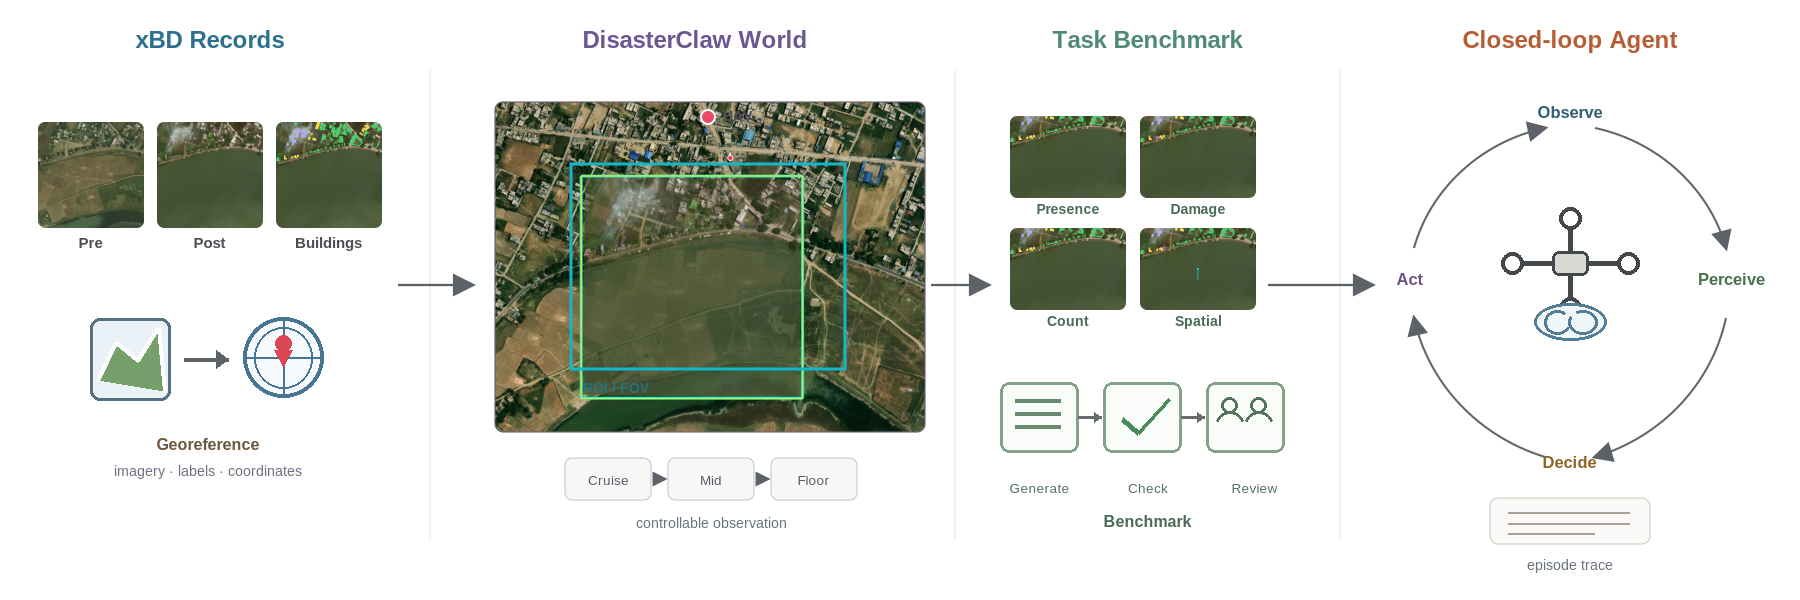
\includegraphics[width=\linewidth]{figure-paper/Fig_DisasterClaw_Refined_NoOverlap.png}
\caption{Data-to-episode workflow in DisasterClaw. Paired xBD imagery and building annotations provide a geographic scene and reference evidence; map anchoring makes observations depend on vehicle state; task generation, checks, and review produce a frozen benchmark; the platform records closed-loop inspection episodes. Image panels illustrate these stages rather than documenting one final-test trajectory.}
\label{fig:overview}
\end{figure}

Table~\ref{tab:platform} states what each layer implements and the boundary attached to it. This distinction is central to the intended use of the platform. Its geospatial state and image renderer support controlled observation studies; they do not reproduce the complete physics of an aircraft or camera.

\begin{table}[htbp]
\centering\footnotesize
\caption{Implemented DisasterClaw capabilities and their evaluation boundaries.}
\label{tab:platform}
\begin{tabularx}{\linewidth}{@{}>{\raggedright\arraybackslash}p{2.25cm}>{\raggedright\arraybackslash}X>{\raggedright\arraybackslash}X@{}}
\toprule
Capability & Implemented function & Boundary in this study \\
\midrule
Scene & Georeferenced pre-/post-disaster tiles, building annotations, map anchors, target ROIs, and contextual basemap & Three evaluated events and 44 ROIs; incomplete source archive and no global coverage claim \\
Observation & Nadir fixed-FOV crop and resampling at three footprint widths; paired archival and current-image channels & Orthographic imagery; no new viewpoint, acquisition time, or detail below the assumed 0.5 m/pixel source scale \\
Vehicle and actions & Geographic and local position, altitude, heading, speed, task state, straight-line motion, centering, descent, hover, marking, and reporting & One UAV with simplified kinematics; no six-degree-of-freedom dynamics, wind, collision, communication, or battery model \\
Perception and models & Building localization and binary no-damage/damaged evidence, geographic cross-view evidence memory, task-specific spatial summaries, and Qwen answer generation & Fixed ChangeOS backend with prior xBD exposure; fixed Qwen2.5-VL-7B-Instruct answer model; no claim of event-disjoint perception generalization \\
Tasks & Operator instructions, damage/presence/count/spatial questions, and archived language-guided navigation instructions & Task-scoped simulation; no claim of unrestricted natural-language or open-world competence \\
Logging and evaluation & Interactive monitoring, headless episodes, paired task IDs, intermediate evidence, actions, budgets, answers, and terminal scores & All 3,360 final online episodes are covered by local shard-level consistency audits; complete public release packaging remains pending \\
Physical boundary & Map-anchored scene transitions and a controlled observation ladder & No photorealistic sensor synthesis, aircraft certification model, hardware-in-the-loop result, or physical-flight validation \\
\bottomrule
\end{tabularx}

\end{table}

The design has three objectives: retain the geographic relationship between source imagery and inspection targets, expose a controllable observation through a common agent interface, and preserve the evidence needed to reconstruct task outcomes. The benchmark is constructed from the same registered source records, but its reference annotations are kept separate from agent observations. This separates world construction, answer construction, and policy execution.

\subsection{Map-anchored disaster-world construction}
The scene layer reads paired pre- and post-disaster tiles, building polygons, damage labels, and geographic metadata derived from xBD. Pixel-to-geographic and geographic-to-pixel affine transforms place each image on its recorded ground footprint. When a tile becomes active, its center defines the local world anchor. Robot, target, and report coordinates remain available as latitude, longitude, and altitude, while local north and east offsets are recomputed relative to that anchor.

The interactive map can place the active disaster image over a satellite or street basemap, display the tile boundary, and color annotated buildings for operator reference. These annotation overlays are not passed to the evaluated agent as visual input. In rendered observations, georeferenced disaster tiles supply task evidence and the surrounding basemap supplies spatial context when a wider footprint extends beyond the available disaster tile. Reference answers and building-level scores remain restricted to the annotated target ROI, so contextual background is not treated as disaster ground truth.

The evaluated scene population contains three disaster events and 44 target ROIs. This is the experimental subset, not a claim that the software can reproduce every disaster represented by the source dataset. Missing tiles, sparse geographic coverage, affine-registration error, and differences in acquisition date all constrain the resulting environment.

\begin{figure}[htbp]
\centering
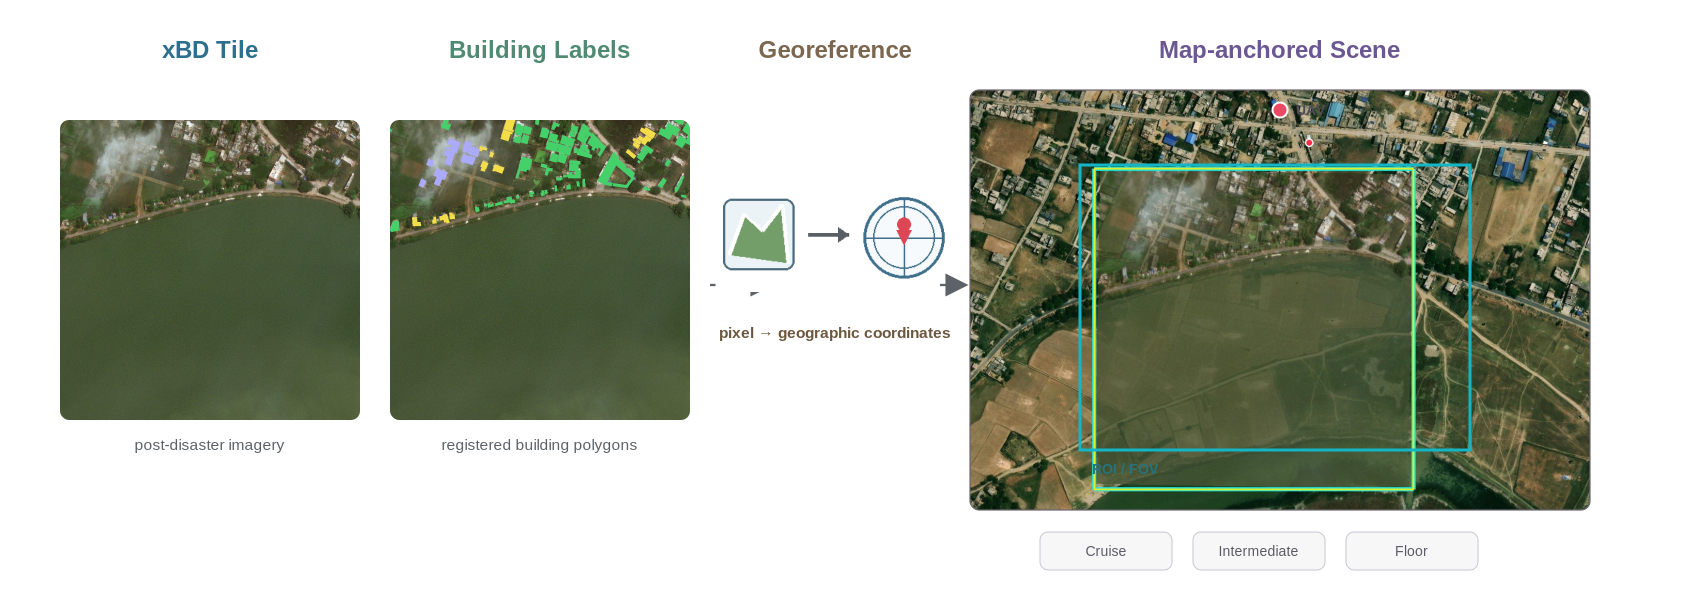
\includegraphics[width=\linewidth]{figure-paper/Fig2_MapAnchored_Integration.png}
\caption{Geographic embedding of disaster records. Image footprints and building polygons are placed in a shared map coordinate system, allowing the environment to associate observations and target locations with geographic state. The supplied visualization illustrates registration and overlays; its colors and markers are not a verified final-task answer key. Basemap context outside the annotated ROI does not supply disaster ground truth.}
\label{fig:map-anchored}
\end{figure}

\subsection{Controllable observation model}
The simulated sensor is nadir-facing, with horizontal field of view $\theta$ and fixed output width $W$. For vehicle height $h$, the ground-footprint width $L$ and effective ground sampling distance $g$ are
\begin{equation}
 L(h)=2h\tan(\theta/2),\qquad g(h)=\frac{L(h)}{W}.
 \label{eq:geometry}
\end{equation}
We use $\theta=60^\circ$, $W=1024$, and an assumed source scale of $0.5$ m/pixel. A $1024$-pixel source tile therefore spans 512 m. Footprints of three, two, and one tile widths define cruise, intermediate, and floor states at approximately 1330.2, 886.8, and 443.4 m, with effective GSDs of 1.5, 1.0, and 0.5 m/pixel (Fig.~\ref{fig:ladder}). The heights are derived parameters of this camera abstraction; they are not measured flight altitudes from the source imagery.

\begin{figure}[htbp]
\centering
\resizebox{\linewidth}{!}{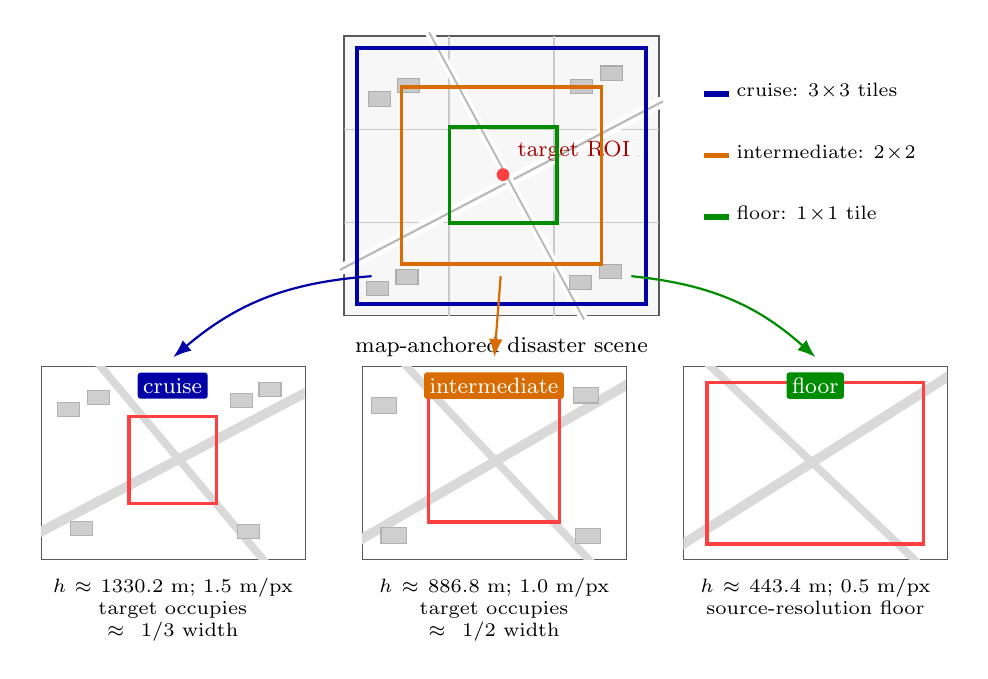
\begin{tikzpicture}[
  font=\footnotesize,
  >=Latex,
  view/.style={draw=black!65,minimum width=3.35cm,minimum height=2.45cm,inner sep=0pt},
  note/.style={align=center,text width=3.45cm,font=\scriptsize}
]
% Source mosaic and nested ground footprints.
\begin{scope}[shift={(3.85,3.55)}]
  \draw[fill=gray!6,draw=black!65] (0,0) rectangle (4.0,3.55);
  \foreach \x in {1.333,2.667}{\draw[gray!42] (\x,0)--(\x,3.55);}
  \foreach \y in {1.183,2.367}{\draw[gray!42] (0,\y)--(4,\y);}
  \draw[line width=4pt,white] (-.05,.58)--(4.05,2.72);
  \draw[line width=.8pt,gray!55] (-.05,.58)--(4.05,2.72);
  \draw[line width=3.2pt,white] (3.05,-.05)--(1.08,3.60);
  \draw[line width=.7pt,gray!55] (3.05,-.05)--(1.08,3.60);
  \foreach \p in {(.45,2.75),(.82,2.92),(3.02,2.91),(3.40,3.08),(3.00,.42),(3.38,.56),(.43,.34),(.80,.49)}{
    \draw[fill=gray!42,draw=gray!65] \p ++(-.14,-.09) rectangle ++(.28,.18);
  }
  \fill[red!75] (2.02,1.79) circle (2.3pt);
  \node[red!65!black,anchor=south west] at (2.08,1.84) {target ROI};
  \draw[line width=1.4pt,blue!65!black] (.17,.15) rectangle (3.83,3.40);
  \draw[line width=1.4pt,orange!85!black] (.73,.65) rectangle (3.27,2.90);
  \draw[line width=1.4pt,green!55!black] (1.34,1.18) rectangle (2.70,2.39);
  \node[anchor=north] at (2,-.15) {map-anchored disaster scene};
\end{scope}

\node[anchor=west,align=left,font=\scriptsize] at (8.30,6.40) {\textcolor{blue!65!black}{\rule{9pt}{2pt}} cruise: $3\!\times\!3$ tiles};
\node[anchor=west,align=left,font=\scriptsize] at (8.30,5.62) {\textcolor{orange!85!black}{\rule{9pt}{2pt}} intermediate: $2\!\times\!2$};
\node[anchor=west,align=left,font=\scriptsize] at (8.30,4.84) {\textcolor{green!55!black}{\rule{9pt}{2pt}} floor: $1\!\times\!1$ tile};

% Three observations have the same output size.
\begin{scope}[shift={(0,0.45)}]
  \node[view,anchor=south west] at (0,0) {};
  \clip (0,0) rectangle (3.35,2.45);
  \draw[line width=3.5pt,gray!30] (-.2,.25)--(3.55,2.22);
  \draw[line width=2.8pt,gray!30] (2.95,-.15)--(.62,2.62);
  \foreach \p in {(.35,1.91),(.73,2.06),(2.55,2.02),(2.91,2.16),(2.64,.36),(.52,.40)}{
    \draw[fill=gray!38,draw=gray!60] \p ++(-.14,-.09) rectangle ++(.28,.18);
  }
  \draw[very thick,red!75] (1.12,.71) rectangle (2.23,1.82);
  \node[fill=blue!65!black,text=white,rounded corners=1pt,inner sep=2pt] at (1.675,2.21) {cruise};
\end{scope}
\node[note,anchor=north] at (1.675,.34) {$h\approx1330.2$ m; 1.5 m/px\\target occupies $\approx1/3$ width};

\begin{scope}[shift={(4.08,0.45)}]
  \node[view,anchor=south west] at (0,0) {};
  \clip (0,0) rectangle (3.35,2.45);
  \draw[line width=3.5pt,gray!30] (-.25,.12)--(3.6,2.36);
  \draw[line width=2.8pt,gray!30] (3.05,-.18)--(.40,2.63);
  \foreach \p in {(.28,1.96),(2.84,2.09),(2.87,.30),(.40,.31)}{
    \draw[fill=gray!38,draw=gray!60] \p ++(-.16,-.10) rectangle ++(.32,.20);
  }
  \draw[very thick,red!75] (.84,.48) rectangle (2.51,2.15);
  \node[fill=orange!85!black,text=white,rounded corners=1pt,inner sep=2pt] at (1.675,2.21) {intermediate};
\end{scope}
\node[note,anchor=north] at (5.755,.34) {$h\approx886.8$ m; 1.0 m/px\\target occupies $\approx1/2$ width};

\begin{scope}[shift={(8.16,0.45)}]
  \node[view,anchor=south west] at (0,0) {};
  \clip (0,0) rectangle (3.35,2.45);
  \draw[line width=3.5pt,gray!30] (-.35,-.02)--(3.7,2.54);
  \draw[line width=2.8pt,gray!30] (3.18,-.23)--(.12,2.67);
  \draw[very thick,red!75] (.30,.20) rectangle (3.05,2.25);
  \node[fill=green!55!black,text=white,rounded corners=1pt,inner sep=2pt] at (1.675,2.21) {floor};
\end{scope}
\node[note,anchor=north] at (9.835,.34) {$h\approx443.4$ m; 0.5 m/px\\source-resolution floor};

\draw[->,thick,blue!65!black] (4.20,4.05) to[bend right=18] (1.68,3.02);
\draw[->,thick,orange!85!black] (5.84,4.05) -- (5.76,3.02);
\draw[->,thick,green!55!black] (7.50,4.05) to[bend left=18] (9.84,3.02);
\end{tikzpicture}
}
\caption{Observation construction from one georeferenced scene. Each state is rendered to $1024\times1024$ pixels. Descending narrows the ground footprint and assigns more existing source pixels to the target ROI; the floor state reaches, but cannot exceed, the assumed source resolution.}
\label{fig:ladder}
\end{figure}

For paired damage perception, the post-disaster channel is sampled at the current footprint and fixed output size. The corresponding pre-disaster window is retained at the assumed source scale before the pair is brought to the detector input geometry. This represents access to an archival reference and a controllable current observation. It also means the two channels undergo different resampling. The platform records this choice because it can contribute to any observed view response.

Changing height only crops and resamples existing orthographic imagery. The renderer does not create sub-source detail, oblique views, three-dimensional parallax, self-occlusion, atmospheric effects, motion blur, or a new acquisition time. At the floor, further descent cannot add information under the adopted source model.

\subsection{Agent--environment interaction interface}
The world model stores a single UAV with geographic position, altitude, heading, speed, flight status, and task state. It also stores targets, reports, the active disaster tile, map bounds, and timestamps. Motion is implemented by straight-line interpolation in a locally anchored horizontal frame. A position update is converted between geographic coordinates and local north--east offsets, and altitude is recorded as the vertical state.

The task planner and closed-loop agent share a finite set of environment tools: fly to a geographic coordinate, move by a relative horizontal or vertical offset, hover, run disaster detection, mark a target, and produce a report. The inspection controller additionally uses answer, abstain, and stop as episode decisions. A reobservation maps to one or more movement primitives, such as centering on evidence and descending by one camera-ladder state, followed by a new render and perception pass.

This action model supports repeatable studies of where the sensor is pointed and how often another observation is requested. It omits rigid-body attitude dynamics, acceleration limits, wind, terrain following, collision checking, communications, and battery discharge. Executed action count is therefore the principal online cost in this paper. Any time estimate obtained from configured speeds remains a simulator quantity rather than measured endurance.

\subsection{Instrumentation and benchmark execution}
The console exposes disaster selection, a georeferenced situation map, manual flight controls, language-task submission, perception displays, agent state, and event logs. An operator can activate a disaster tile, select a target location, issue an inspection task, observe the planned or closed-loop actions, and inspect the returned damage evidence. The operator console supports qualitative inspection of the same scene state, perception evidence, decisions, actions, budgets, and event logs used by the headless benchmark. The interface is intended for monitoring and diagnosis; all quantitative results in this study are produced by the frozen headless protocol.

The headless benchmark initializes a question and vehicle state, invokes the same observation and action modules, and writes the evolving answer, evidence, controller decision, movement, budget, and terminal outcome. Frozen question identifiers allow policies to be compared on paired tasks. The implementation also supports a fixed-view mode that holds the environment state constant while repeating answer generation. The final benchmark binds generation seeds to question, repeat, step, and call role, making environmental changes and subsequent generation calls separately traceable. Policies may still make different numbers of later calls, so whole-policy comparisons are not pure action-only effects.

\begin{figure}[htbp]
\centering
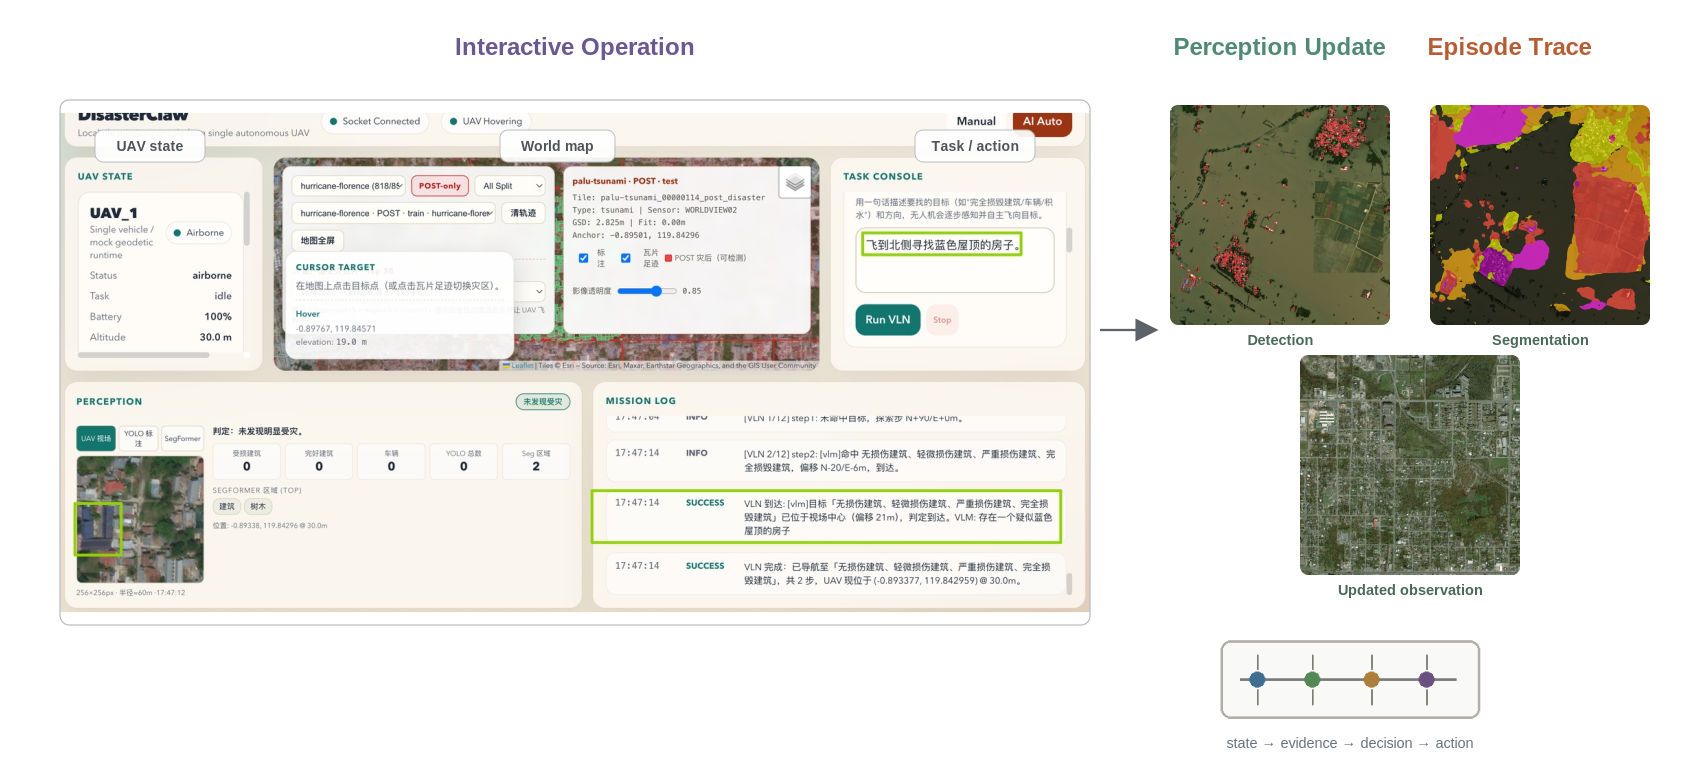
\includegraphics[width=\linewidth]{figure-paper/Fig4_ClosedLoop_Platform.png}
\caption{Representative console, perception displays, and closed-loop instrumentation. This supplied composite shows general platform interfaces, including legacy YOLO/SegFormer and VLN controls; it is not a single synchronized episode or a screenshot of the frozen ChangeOS experiment. The displayed 30 m setting is an interface example, not a height used in the camera-ladder evaluation. Quantitative results use the headless protocol described in Section~\ref{sec:setup}.}
\label{fig:console}
\end{figure}

\section{Closed-loop inspection and observation rules}
\label{sec:agent}
\subsection{Task, state, and evidence}
Each inspection episode has a question $q$, a geographic region of interest (ROI), a task type (presence, damage, count, or spatial relation), and a reference answer $y_q$. At step $t$, the simplified vehicle state $s_t=(x_t,y_t,h_t)$ determines a rendered image $I_t=\mathcal{R}(\mathcal{M},s_t)$ from scene $\mathcal{M}$. The agent also receives structured evidence $z_t$ from the fixed perception backend and registered environment state. It may search, request a task-appropriate reobservation, answer, abstain, or stop. A reobservation is counted only when a movement executes and a new view is rendered; a repeated answer on an unchanged view is not an observation action.

Figure~\ref{fig:agent-loop} summarizes the agent loop. The benchmark retains the intermediate answer, decision, movement, evidence, generation-call keys, and terminal outcome. It scores the terminal normalized answer against $y_q$, with abstentions counted as unsuccessful answers. This is an episode-level question-answering endpoint rather than an average of building classifications.

\begin{figure}[htbp]
\centering
\resizebox{\linewidth}{!}{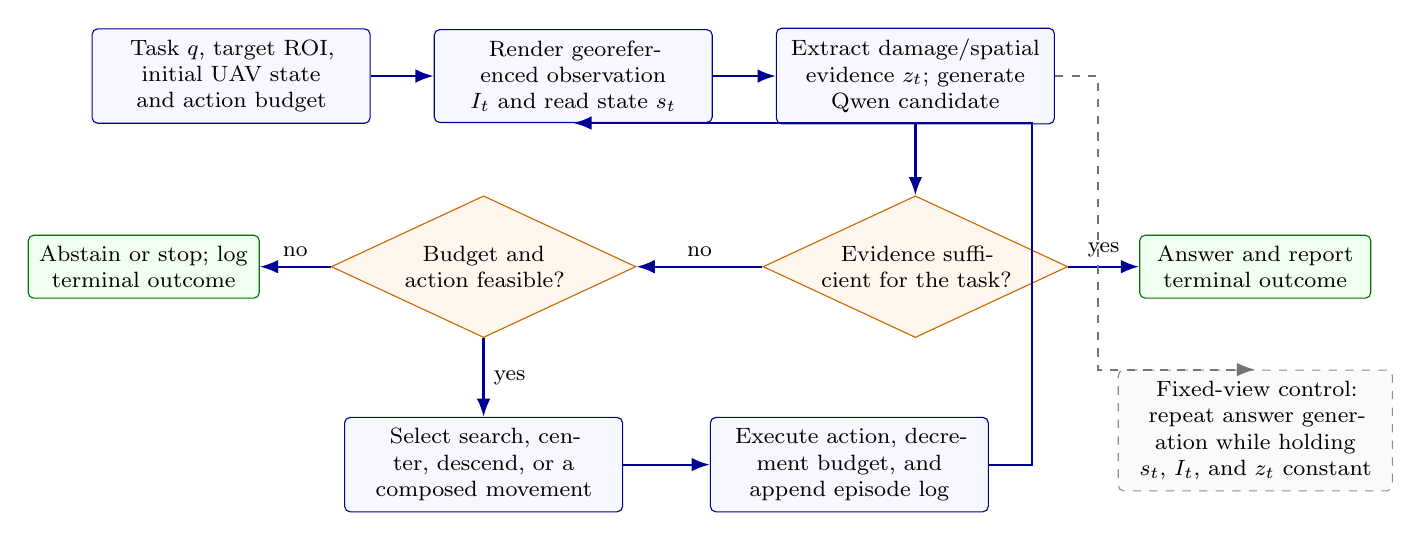
\begin{tikzpicture}[
  font=\footnotesize,
  >=Latex,
  state/.style={draw=blue!58!black,rounded corners=2pt,fill=blue!3,align=center,
    text width=3.25cm,minimum height=.88cm,inner sep=4pt},
  decision/.style={diamond,draw=orange!80!black,fill=orange!7,aspect=2.15,
    align=center,text width=2.4cm,inner sep=1.5pt},
  terminal/.style={draw=green!45!black,rounded corners=2pt,fill=green!6,align=center,
    text width=2.7cm,minimum height=.8cm},
  arr/.style={->,thick,draw=blue!58!black},
  control/.style={draw=black!45,dashed,rounded corners=2pt,fill=gray!4,align=center,
    text width=3.2cm,inner sep=4pt}
]
\node[state] (init) {Task $q$, target ROI, initial UAV state and action budget};
\node[state,right=8mm of init] (render) {Render georeferenced observation $I_t$ and read state $s_t$};
\node[state,right=8mm of render] (infer) {Extract damage/spatial evidence $z_t$; generate Qwen candidate};
\node[decision,below=9mm of infer] (enough) {Evidence sufficient for the task?};
\node[terminal,right=9mm of enough] (answer) {Answer and report terminal outcome};
\node[decision,left=16mm of enough] (feasible) {Budget and action feasible?};
\node[terminal,left=9mm of feasible] (abstain) {Abstain or stop; log terminal outcome};
\node[state,below=10mm of feasible] (choose) {Select search, center, descend, or a composed movement};
\node[state,right=11mm of choose] (execute) {Execute action, decrement budget, and append episode log};
\node[control,below=9mm of answer] (fixed) {Fixed-view control: repeat answer generation while holding $s_t$, $I_t$, and $z_t$ constant};

\draw[arr] (init)--(render);
\draw[arr] (render)--(infer);
\draw[arr] (infer)--(enough);
\draw[arr] (enough)--node[above]{yes}(answer);
\draw[arr] (enough)--node[above]{no}(feasible);
\draw[arr] (feasible)--node[above]{no}(abstain);
\draw[arr] (feasible)--node[right]{yes}(choose);
\draw[arr] (choose)--(execute);
\draw[arr] (execute.east) -- ++(.55,0) |- (render.south);
\draw[->,thick,dashed,draw=black!55] (infer.east) -- ++(.55,0) |- (fixed.north);
\end{tikzpicture}
}
\caption{Closed-loop inspection state machine. Feasibility and budget checks distinguish a requested reobservation from an executed view change. The unchanged-view branch is available for diagnosis but is not counted as reobservation.}
\label{fig:agent-loop}
\end{figure}

\subsection{Fixed binary perception and cross-view memory}
The main experiments use the same frozen ChangeOS ResNet-34 checkpoint for every policy. It detects buildings in registered pre-/post-disaster imagery and supplies a binary no-damage/damaged probability vector. ChangeOS is an external perception tool, not a newly trained contribution of this study. Its checkpoint has prior xBD exposure; neither the perception evaluation nor the online results demonstrate transfer of the detector to unseen disaster events.

For a binary vector $p_i=(p_{i0},p_{i1})$, the damage-uncertainty score is
\begin{equation}
 H_2(p_i)=-\frac{1}{\log 2}\sum_{j=0}^{1}p_{ij}\log p_{ij}.
 \label{eq:entropy}
\end{equation}
The raw-entropy policy uses the uncalibrated binary probabilities, whereas calibrated entropy and a prediction-set trigger are supplemental comparisons. Historical four-class temperature and APS thresholds are not transferred to this experiment. For count tasks, the task-conditioned gate estimates uncertainty over the answer buckets $0,1,2,3+$ from the binary building probabilities; for spatial tasks it uses registered target geometry and a GSD-dependent bearing uncertainty. Thus a single uncertain building label is not treated as a sufficient reason to crop away a complete count or spatial ROI.

The online evidence memory matches predicted objects by geographic proximity and combines observations across views, preserving the history of observation IDs and ROI coverage. This avoids treating each new crop as an unrelated scene or automatically discarding earlier wide-view evidence. Answer generation uses a locally loaded Qwen2.5-VL-7B-Instruct model with the task image and selected structured state; the evaluated configurations use the same hybrid answer path. The model's output is normalized to the task's answer vocabulary before scoring. A deterministic rule answerer and pure-VLM paths exist as development diagnostics, but are not pooled into the seven-policy final comparison.

\subsection{Task-conditioned gate and comparators}
The task-conditioned policy (T1\_TASK) estimates whether an executable next view is worth its cost. In its implemented rule, the candidate utility is
\begin{equation}
 U_q= u_q(1-h_{t+1}/h_t)
 -0.05\,\widehat{T}_{\mathrm{move}}/60
 -(1-\widehat{C}_{\mathrm{ROI}}),
 \label{eq:taskutility}
\end{equation}
where $u_q$ is task-specific uncertainty, $\widehat{T}_{\mathrm{move}}$ is a configured-speed motion-time estimate in seconds, and $\widehat{C}_{\mathrm{ROI}}$ is predicted ROI coverage after the candidate action. This is a fixed heuristic, not a learned or calibrated estimate of expected task accuracy. The frozen gate requires $u_q\geq0.5$ and $U_q\geq0.05$; count and spatial tasks additionally require predicted coverage of at least 0.98. A damage question may center on a visible marked target and descend. Count and spatial questions retain the geographic center and descend only if the task ROI remains covered. Presence positives are answered from the wide view, while missing evidence uses the search path. All thresholds were chosen before the final run using development evidence.

The four primary comparators are A0\_HOLD (search allowed, no reobservation), A1\_RANDOM (independent seeded random trigger), A2\_ALWAYS (request whenever feasible), and A3U\_RAW\_ENTROPY (binary raw-entropy trigger). A3\_ENTROPY and A4\_CONFORMAL are supplemental. Each active policy has the same exogenous cap of two reobservations per episode, and all configurations permit up to six search steps. A0\_HOLD has a zero reobservation cap. The cap is shared, but realized action counts differ because policy requests and feasibility differ; the seven outcomes are operating points, not a randomized budget sweep.

\section{Experimental protocol}
\label{sec:setup}
\subsection{Development diagnostics and frozen final tasks}
The ChangeOS camera-ladder diagnostic uses 43 development ROIs containing 7,238 annotated buildings. It compares cruise, intermediate, and floor predictions on the same ground-truth building identities. The full-ground-truth endpoint counts an unmatched building as incorrect; matched-only classification and probability metrics use only matched detections. These are development and mechanism measurements, not final policy scores.

The confirmatory online question set is separate from the 160-question development set used to choose policy rules. It contains 160 questions from 44 previously unconsumed ROIs: 48 in Hurricane Michael, 51 in the Moore tornado, and 61 in Nepal flooding. Questions cover presence, damage, count, and spatial relations. The author manually reviewed all 160 and approved the frozen set; 88 previously flagged ambiguity notices remain recorded rather than erased. The present record documents one author's review, not two independent annotators or an inter-rater agreement estimate. The final question set, review report, binary-label manifest, and source/prompt/weight hashes were checked before the first online episode. The exact identities and checksums are listed in Appendix~\ref{app:provenance}.

\subsection{Online execution and endpoints}
Seven policies run on each of the 160 final questions for each of three generation repeats, producing 3,360 planned episodes. Four shards partition each repeat without changing the question set. The action base seed is 42; generation calls derive their seed from base 42000 and $(\mathrm{qid},\mathrm{repeat},\mathrm{step},\mathrm{call\ role})$. Qwen sampling settings, source fingerprint, prompt hash, and ChangeOS weights are frozen in the protocol. All 12 shard audits passed with zero execution errors. Repeats provide three generation conditions on the same 160 questions; they are not new independent questions, ROIs, or events.

The prespecified primary endpoint is terminal task accuracy over all questions, averaged over repeats. Abstentions count as incorrect for this endpoint. Secondary descriptions include accuracy by event and task type, abstention, within-policy answer correction and harm, executed reobservations, state-derived horizontal/vertical motion, and episode wall time. A correction or harm observed inside one policy's trajectory is not the counterfactual effect of its action relative to another policy. Later VLM call counts can also differ across policies, so paired accuracy contrasts estimate whole-policy outcomes rather than a pure image-change effect.

Four T1\_TASK contrasts against A0\_HOLD, A1\_RANDOM, A2\_ALWAYS, and A3U\_RAW\_ENTROPY were declared before execution. Pairing uses the same $(\mathrm{repeat},\mathrm{qid})$ units. For each contrast, a 5,000-draw ROI-cluster bootstrap resamples all questions and three repeats within each sampled ROI, with seed 42. The four primary comparisons use Bonferroni-adjusted 98.75\% percentile intervals; 95\% intervals are descriptive. Only three events are represented, so these intervals characterize variation among the observed ROI clusters, not transfer to unseen disasters. Event and question-type breakdowns are descriptive rather than additional confirmatory tests.

Executed reobservation count is the principal observed action-cost measure. Episode wall time is measured software runtime for this execution, not UAV flight time. Trajectory-state displacements are geometric estimates, and configured-speed $d/v$ values are estimates rather than measured airborne duration. No randomized common-cap sweep or component-level render/ChangeOS/controller/Qwen timing is available. Accordingly, accuracy and cost are reported as realized policy operating points.

\section{Results and discussion}
\subsection{RQ1: A narrower observation changes both detection and correctness}
The development camera-ladder diagnostic keeps 7,238 ground-truth buildings in 43 ROIs fixed while changing the rendered footprint. ChangeOS localization recall rises from 22.09\% at cruise to 34.06\% at intermediate and 56.52\% at floor. When unmatched ground-truth buildings are counted as incorrect, binary accuracy rises from 20.01\% to 31.06\% and 53.65\%, respectively. Among matched buildings alone, accuracy is 90.56\%, 91.20\%, and 94.92\%, with macro-F1 of 0.8714, 0.8743, and 0.9232. Matched-only Brier score falls from 0.0657 to 0.0384 between cruise and floor; these probability metrics are not defined over unmatched ground-truth buildings. The large gap between all-GT and matched-only accuracy shows that localization and observation coverage, not just binary classification, dominate the full-building endpoint. Because matched populations change by view, their classification percentages must not replace the fixed-denominator measure.

For the paired cruise-to-floor comparison, 2,696 building outcomes change from incorrect to correct and 261 change from correct to incorrect, a net gain of 2,435 on this development population. The same nominally closer view therefore supplies useful detail and harmful changes. These are binary ChangeOS diagnostics; the archived four-class results in \ref{app:historical} belong to a different backend and are not pooled with them. More importantly, building-level gains do not by themselves imply better task answers.

\subsection{RQ2 and RQ3: Frozen online policies and task answers}
Table~\ref{tab:final-policies} reports the complete online comparison. T1\_TASK has the highest observed accuracy, 75.00\%, compared with 72.29\% for A0\_HOLD. It uses 161 executed reobservations across 480 question-repeat episodes, compared with 419 for random, 923 for always, and 626 for raw entropy. The higher observed score and lower realized reobservation count are useful descriptive results. They are not a matched-cost comparison: policies have the same maximum cap but choose different numbers of actions.

\begin{table}[htbp]
\centering\small
\caption{Frozen final-set online policies. Each row contains the same 160 questions under three generation repeats (480 question-repeat episodes); repeats are not independent questions. Wall time is measured software episode runtime, not flight duration. A3 and A4 are supplemental comparisons.}
\label{tab:final-policies}
\resizebox{\linewidth}{!}{\begin{tabular}{lrrrr}
\toprule
Policy & Correct / 480 & Accuracy (\%) & Reobservations & Wall time (s/episode)\\
\midrule
A0\_HOLD & 347 & 72.29 & 0 & 17.03\\
A1\_RANDOM & 326 & 67.92 & 419 & 33.65\\
A2\_ALWAYS & 307 & 63.96 & 923 & 51.07\\
A3U\_RAW\_ENTROPY & 339 & 70.63 & 626 & 39.61\\
A3\_ENTROPY & 341 & 71.04 & 628 & 38.94\\
A4\_CONFORMAL & 338 & 70.42 & 628 & 38.95\\
T1\_TASK & 360 & 75.00 & 161 & 17.92\\
\bottomrule
\end{tabular}}
\end{table}

The four prespecified paired contrasts are in Table~\ref{tab:final-contrasts}. T1\_TASK exceeds A0\_HOLD by an observed 2.71 percentage points, but the multiplicity-adjusted ROI-cluster interval includes zero. The appropriate claim is that T1 is higher \emph{in this final run}, while a stable advantage over holding remains uncertain. Its contrast with raw entropy is likewise uncertain. The interval against random touches zero at its lower endpoint, so it does not establish a strict positive difference under the declared interval rule. T1 is above always reobserving within the prespecified cluster analysis, but this comparison alone does not prove that its individual movements caused the gain.

\begin{table}[htbp]
\centering\small
\caption{Prespecified T1\_TASK paired accuracy contrasts. Differences are percentage points; 98.75\% ROI-cluster percentile intervals adjust for the four primary comparisons. All questions and repeats from a sampled ROI remain together.}
\label{tab:final-contrasts}
\begin{tabular}{lrr}
\toprule
Contrast & Difference (pp) & 98.75\% interval (pp)\\
\midrule
T1 minus A0\_HOLD & $+2.71$ & $[-2.04,\,+7.50]$\\
T1 minus A1\_RANDOM & $+7.08$ & $[0.00,\,+14.70]$\\
T1 minus A2\_ALWAYS & $+11.04$ & $[+0.86,\,+21.38]$\\
T1 minus A3U\_RAW\_ENTROPY & $+4.38$ & $[-4.33,\,+12.96]$\\
\bottomrule
\end{tabular}
\end{table}

Additional observations can alter the answer in either direction. Within their own episode histories, T1\_TASK records 36 corrected and 21 harmed answers; A2\_ALWAYS records 74 corrected and 132 harmed. These transition labels are not paired counterfactual effects versus A0\_HOLD. They nevertheless show why an always-reobserve policy can spend the largest action budget while finishing with the lowest accuracy. A1\_RANDOM executes 419 reobservations and reaches 67.92\%; A3U\_RAW\_ENTROPY executes 626 and reaches 70.63\%. Neither action count nor classifier uncertainty alone orders final task quality.

The episode traces show concrete instances in both directions. In the first generation repeat, a Hurricane Michael damage question (ID ending \texttt{damage\_0001\_9430}) changes from an initially incorrect ``no damage'' answer to the correct ``damaged'' answer after two T1 reobservations. A Hurricane Michael spatial question (ID ending \texttt{spatial\_0092\_5452}) changes from the correct ``north'' to the incorrect ``southwest'' after one. These examples describe recorded answer sequences, not isolated causal effects of the movement.

\subsection{RQ4 and RQ5: Task dependence, bottlenecks, and scope of the gain}
Task-type outcomes reveal uneven effects. For T1\_TASK versus A0\_HOLD, damage accuracy is 75.76\% versus 66.67\% and count accuracy is 78.29\% versus 75.97\%. Presence is identical at 93.18\%; spatial accuracy is lower for T1, 41.38\% versus 43.68\%. These are descriptive, correlated subgroup summaries, not four additional adjusted tests. They are consistent with the design premise that a wide context can already suffice for presence while a more detailed target view may help damage, but the spatial result limits any universal benefit claim.

\begin{table}[htbp]
\centering\small
\caption{Task evidence requirements and descriptive final accuracy. A0 and T1 use the same questions and three repeats. The evidence requirements follow the task definitions; they are not experimentally isolated causes of the accuracy differences.}
\label{tab:task-evidence}
\begin{tabularx}{\linewidth}{@{}lXrr@{}}
\toprule
Task & Evidence requirement & A0 (\%) & T1 (\%) \\
\midrule
Presence & Regional coverage and positive evidence & 93.18 & 93.18 \\
Damage & Target identity and local damage detail & 66.67 & 75.76 \\
Count & ROI coverage and consistent object aggregation & 75.97 & 78.29 \\
Spatial & Reference geometry and nearest-target identity & 43.68 & 41.38 \\
\bottomrule
\end{tabularx}
\end{table}

Table~\ref{tab:task-evidence} connects these outcomes to benchmark construction. Narrowing a view allocates more source pixels to a building, but it can remove other buildings needed for a count or the context needed to identify the nearest damaged target. The benchmark therefore exposes competing requirements for detail and coverage rather than ranking every narrower view as better. The platform's joint record of ROI coverage, predicted objects, actions, and answers makes such trade-offs inspectable; it does not by itself resolve their causal contributions.

Event outcomes are also heterogeneous. T1\_TASK versus A0\_HOLD is 54.86\% versus 58.33\% in Hurricane Michael, 84.31\% versus 77.12\% in the Moore tornado, and 83.06\% versus 79.23\% in Nepal flooding. The pooled numerical gain is not reproduced in every event, and three events cannot support an unseen-disaster generalization claim. Accuracy across T1's three generation repeats is 75.00\%, 74.38\%, and 75.63\%; repeat stability does not remove ROI or event uncertainty.

Development diagnostics provide limited bottleneck evidence without forming an additive oracle decomposition. A deterministic answerer using predicted structured evidence reaches 66.87\% on an earlier development run. Full-ROI ground-truth evidence with a deterministic rule answerer reconstructs 160/160 development reference answers, checking the question/label pipeline rather than online performance. Their source fingerprints and interventions differ, and current-visible GT with Qwen, full-task GT with Qwen, and a full-coverage always-floor reference remain unmeasured. The final T1/A0 comparison therefore isolates neither the perception error nor the language-generation error as a unique cause.

The observed T1 operating point combines a modest numerical accuracy gain over holding with fewer executed reobservations than other active policies. Its uncertainty interval, event variation, and incomplete oracle chain favor a platform-and-mechanism interpretation rather than a demonstrated generally superior task-conditioned algorithm. A randomized common-budget sweep would be needed to estimate a genuine accuracy--cost curve; the seven realized operating points cannot supply one by rebinning episodes after execution.

\section{Limitations and deployment boundary}
\label{sec:limitations}
The camera ladder crops and resamples existing orthographic imagery. It changes geographic footprint and assigned source pixels, but it cannot synthesize a new viewing angle, acquisition time, illumination condition, occluded surface, or detail below native resolution. Pre- and post-disaster channels undergo different resampling, and basemap context may come from a different date. The fixed flat-ground, nadir abstraction does not validate altitude-dependent image formation for a physical UAV.

The vehicle model uses simplified position updates without wind, attitude dynamics, acceleration limits, terrain and collision avoidance, communications, or battery discharge. Executed reobservations are measured software actions. State-derived horizontal and vertical displacements are geometric estimates. Of 3,360 final episodes, 42 end with a fly action lacking a subsequent recorded state, so complete-motion summaries are available for 3,318. Episode wall time is measured execution time on the experiment system, not measured flight time; render, ChangeOS, controller, and Qwen component latencies were not separately recorded. No PX4/Gazebo or physical-flight action mapping was performed. The study therefore concerns imagery-grounded active observation, not operational flight performance.

The ChangeOS checkpoint is fixed across policies but has prior exposure to related xBD data; the final policy comparison does not imply event-disjoint perception training. The final questions occupy 44 ROIs in only three disaster events. Although all 160 questions received the author's manual approval before online testing, this is not a two-annotator independent review or an agreement study, and 88 recorded ambiguity notices remain part of the audit trail. Answer frequencies and template families may still permit language-only shortcuts; the same-data development majority and question-only baselines cannot be transported as final-set estimates.

The generation protocol gives three seeded repeats, but active policies can make different numbers of later Qwen calls. Their paired outcomes thus compare entire decision pipelines rather than the isolated causal effect of one movement. The seven policies share a maximum reobservation cap, not equal executed action counts. No randomized cap sweep, full module-level timing, or complete layered GT/Qwen oracle suite is available. The interval for T1\_TASK versus A0\_HOLD includes both a small disadvantage and a useful advantage, and one of three event directions is negative. These boundaries preclude claiming stable superiority over holding or generalization to unseen disasters from the present sample.

Archived four-class allocation and VLN component results in Appendix~\ref{app:historical} use different populations and/or an earlier observation stack. They are historical diagnostics, not replications of the binary ChangeOS final experiment, and their calibration constants or performance numbers are not transferred into the main evidence chain.

\section{Conclusion}
DisasterClaw connects disaster records, an interactive geographic world, a task benchmark, and traceable closed-loop inspection. Paired xBD images and building annotations are anchored to map coordinates shared by the vehicle, observation footprint, and task ROI. Programmatic rules derive presence, damage, count, and spatial questions with annotation- and geometry-based answers; automated checks and dual review produce 160 final tasks over 44 ROIs in three events. A shared console and headless interface then record how an agent's movement changes its observation, perception evidence, and terminal answer. This data-to-world-to-benchmark construction is the principal contribution.

In 160 dual-reviewed final questions over three generation repeats, T1\_TASK reaches 75.00\% accuracy versus 72.29\% for holding and executes fewer reobservations than the other active policies. This is an observed improvement in the tested sample, not an established stable advantage over no reobservation: the prespecified adjusted interval for the 2.71-point difference spans zero. The always-reobserve policy uses 923 actions and finishes at 63.96\%, illustrating that more observation can also be harmful. Together with the development camera-ladder's corrections and harms, these results support the platform's role in measuring task-dependent observation value.

The benchmark makes differing evidence needs explicit: damage assessment can benefit from target detail, while counts and spatial relations also depend on regional coverage and reference geometry. The observed task and event variation supports studying those requirements separately, not recommending one observation policy universally. The next scientific steps are a randomized common-budget comparison, fuller oracle decomposition, component-level timing, independently reviewed questions across more events, and a perception checkpoint evaluated without event exposure. Claims about real flight require external action and imaging validation. Until then, DisasterClaw provides an imagery-grounded platform and benchmark with explicitly bounded evidence, not a demonstrated general-purpose flight policy.

\section*{Declarations for author completion}
\noindent\textbf{Acknowledgements and funding.} \textit{To be supplied by the authors, including funder names, grant numbers, and relevant contributions. No absence of funding is asserted.}

\smallskip\noindent\textbf{CRediT author statement.} \textit{To be assigned and approved by the named authors.}

\smallskip\noindent\textbf{Declaration of competing interest.} \textit{To be confirmed by all authors.}

\smallskip\noindent\textbf{Data and code availability.} The working package contains manuscript source, frozen P6 protocol and hashes, audited final episode logs, and analysis scripts. Access to the underlying imagery remains subject to its original terms. A public archive, license, anonymization review, and complete imagery/checkpoint package have not yet been confirmed; a final availability statement must identify the actual release and its restrictions.

\smallskip\noindent\textbf{Generative AI assistance.} Generative AI tools were used to assist manuscript restructuring, English-language editing, reference checking, and preparation of analysis and typesetting scripts. All scientific claims, experimental design, reported results, and final manuscript content were reviewed and approved by the authors, who take full responsibility for the work.

\appendix
\setcounter{table}{0}
\renewcommand{\theHtable}{A.\arabic{table}}
\section{Reproducibility and provenance}
\label{app:provenance}
\subsection{Frozen final identities and audit boundary}
The final protocol is stored in \path{cja_en/review/changeos_p6_final_protocol_20260915.json}. It records full SHA-256 values for the final task set, a review report, the frozen three-event manifest, ChangeOS weights, source fingerprint, system prompt, policy configuration, and analysis scripts. Its own SHA-256 begins \texttt{41ccbb5fed5e}; exact paths and full hashes are retained in the machine-readable protocol rather than truncated in the audit. These identities describe the local execution; they are not substitutes for a publicly recoverable image and checkpoint package.

The dual-review procedure described in Section~\ref{sec:benchmark} requires two independent review records and an adjudication record linked to the frozen question identifiers. The available protocol lists one review-report path and hash; it does not separately identify those three records. Their inclusion and explicit mapping to the frozen set remain requirements for a complete release. This distinction prevents the execution audit from being interpreted as independent verification of the human-review process. Review records are provenance, not model inputs.

The 12 final shard directories contain manifests, preflight receipts, \path{episodes.jsonl}, \path{results.json}, and strict per-shard audits. Their combined report is \path{p6_final_three_event_v1_20260915_report.json} under \path{runs/benchmarks/changeos_binary/}; its SHA-256 begins \texttt{9e4370325bc9}. It validates 3,360 rows with zero execution errors, exact question/configuration/repeat coverage, and declared input identities. This is a local execution and consistency audit, not an independent re-execution of the full model pipeline. The run uses a fixed ChangeOS checkpoint and a locally loaded Qwen2.5-VL-7B-Instruct model; checkpoint identity and generation settings must accompany any release rather than be inferred from an online model name.

Scene construction and rendering are in the \path{backend/} modules \path{world.py}, \path{geo.py}, \path{xbd_map.py}, \path{fov_ladder.py}, and \path{perception.py}. Inspection, reobservation, and local Qwen calls are in the same directory's \path{agent_vqa.py}, \path{recheck.py}, and \path{local_qwen_vl.py}. The headless protocol is under \path{scripts/benchmarks/}; this directory also contains \path{build_roi_index.py}, \path{gen_agent_vqa_testset_v2.py}, and \path{review_agent_vqa_testset.py} for coverage indexing, task generation, and review checks. The operator interface is under \path{frontend/src/}. This file map establishes software correspondence, not that every optional module was active in each policy.

The final cost audits are \path{runs/benchmarks/changeos_binary/p7_cost_observability_final_repeat0_20260917/report.json}, with corresponding repeat1 and repeat2 paths. The existing auditor was applied to four shards at a time because its duplicate key is not repeat-aware. Together the three reports cover 3,360 episodes and flag 42 incomplete terminal-motion traces. All logged recheck request, inferred allocation, execution, and episode totals agree. Search-action allocation details, component-level timing, actual flight time, and physical action mapping remain unavailable. A complete public reproduction package would additionally need the licensed source imagery, scene manifests and affine transforms, basemap availability, dependency lock, checkpoint retrieval instructions, and one replay with action/observation hashes.

\section{Historical diagnostics outside the main evidence chain}
\label{app:historical}
\subsection{Archived four-class camera and allocation study}
An earlier \texttt{xview2\_first} four-class pipeline evaluated 3,753 buildings in 44 ROIs. It is not the binary ChangeOS backend of the final study. Table~\ref{tab:fov} retains its camera-footprint results and Table~\ref{tab:allocation} its offline allocation at a 0.25 building-selection fraction. The old temperature, prediction-set threshold, four-class entropy normalization, and allocation scores are not used in the main experiment. These offline selections operate on paired stored predictions, not on executable closed-loop routes or question answers.

\begin{table}[htbp]
\centering\small
\caption{Historical four-class building-level camera diagnostic on the same 3,753 evaluation buildings. Not comparable to the binary ChangeOS final question endpoint.}
\label{tab:fov}
\input{tables/historical/xview2_first_fov}
\end{table}

\begin{table}[htbp]
\centering\footnotesize
\caption{Historical four-class offline allocation at a 0.25 building-selection fraction. The label-informed row uses evaluation labels and is not deployable.}
\label{tab:allocation}
\input{tables/historical/xview2_first_allocation}
\end{table}

\begin{figure}[htbp]
\centering
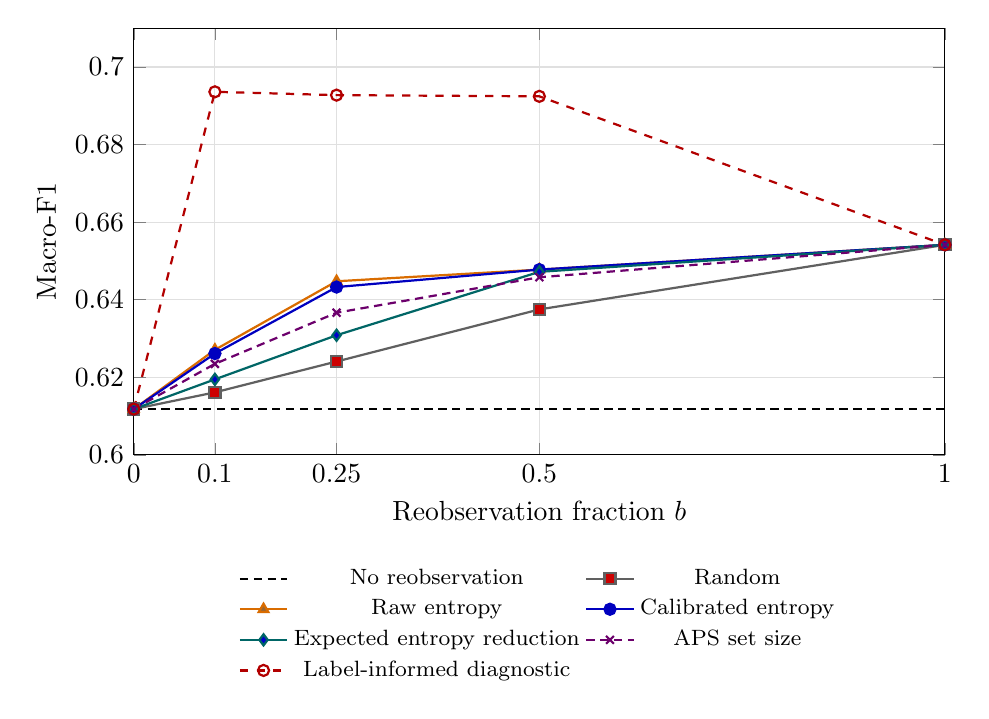
\begin{tikzpicture}
\begin{axis}[
  width=.98\linewidth,height=7.0cm,
  xlabel={Reobservation fraction $b$},ylabel={Macro-F1},
  xmin=0,xmax=1,ymin=.60,ymax=.71,
  xtick={0,.1,.25,.5,1},ytick={.60,.62,.64,.66,.68,.70},
  grid=major,grid style={black!12},
  legend style={at={(.5,-.24)},anchor=north,draw=none,font=\footnotesize},
  legend columns=2,
]
\addplot+[black,densely dashed,mark=none,thick] coordinates {(0,0.61180364) (0.1,0.61180364) (0.25,0.61180364) (0.5,0.61180364) (1,0.61180364)};
\addlegendentry{No reobservation}
\addplot+[gray!75!black,mark=square*,thick] coordinates {(0,0.61180364) (0.1,0.61611550) (0.25,0.62406965) (0.5,0.63750089) (1,0.65415042)};
\addlegendentry{Random}
\addplot+[orange!85!black,mark=triangle*,thick] coordinates {(0,0.61180364) (0.1,0.62708707) (0.25,0.64475982) (0.5,0.64776899) (1,0.65415042)};
\addlegendentry{Raw entropy}
\addplot+[blue!75!black,mark=*,thick] coordinates {(0,0.61180364) (0.1,0.62612436) (0.25,0.64326575) (0.5,0.64776853) (1,0.65415042)};
\addlegendentry{Calibrated entropy}
\addplot+[teal!80!black,mark=diamond*,thick] coordinates {(0,0.61180364) (0.1,0.61946892) (0.25,0.63084430) (0.5,0.64719004) (1,0.65415042)};
\addlegendentry{Expected entropy reduction}
\addplot+[violet!85!black,mark=x,thick] coordinates {(0,0.61180364) (0.1,0.62346363) (0.25,0.63665018) (0.5,0.64578998) (1,0.65415042)};
\addlegendentry{APS set size}
\addplot+[red!70!black,dashed,mark=o,thick] coordinates {(0,0.61180364) (0.1,0.69360303) (0.25,0.69275057) (0.5,0.69243946) (1,0.65415042)};
\addlegendentry{Label-informed diagnostic}
\end{axis}
\end{tikzpicture}

\caption{Historical offline four-class allocation sweep. Selected floor predictions replace cruise predictions; this is not a common-budget online policy curve.}
\label{fig:budget-curve}
\end{figure}

The archived matched-only sensitivity population contains 2,757 buildings detected at all three views (Table~\ref{tab:matched}). Because the subset is selected by detector success, it cannot replace the full 3,753-building endpoint. Its earlier exploratory ROI-bootstrap intervals, shown in Table~\ref{tab:cluster}, condition on fixed scores and the observed three events; they do not demonstrate transfer to new disasters.

\begin{table}[htbp]
\centering\small
\caption{Historical four-class matched-only sensitivity analysis.}
\label{tab:matched}
\begin{tabular}{lrrrr}
\toprule
View & Accuracy & Macro-F1 & Brier & NLL \\
\midrule
Cruise & 0.7918 & 0.7069 & 0.3367 & 0.6455 \\
Mid & 0.8052 & 0.7321 & 0.3176 & 0.6123 \\
Floor & 0.8099 & 0.7489 & 0.3175 & 0.6103 \\
\bottomrule
\end{tabular}

\end{table}

\begin{table}[htbp]
\centering\footnotesize
\caption{Historical four-class exploratory paired ROI-bootstrap differences at the 0.25 offline allocation fraction.}
\label{tab:cluster}
\begin{tabular}{lrr}
\toprule
Paired comparison & Macro-F1 difference & 95\% interval \\
\midrule
Calibrated entropy -- Random & +0.0192 & [+0.0097, +0.0419] \\
Calibrated entropy -- Raw entropy & -0.0015 & [-0.0093, +0.0061] \\
\bottomrule
\end{tabular}

\end{table}

\subsection{Archived VLN switch diagnostic}
The earlier 200-instruction VLN switch experiment used an earlier observation stack and one recorded run per configuration. Table~\ref{tab:vln-ablation} preserves the archived aggregate as a component diagnostic only. Enabling the recheck configuration did not cause recheck actions in that run; the table cannot establish a benefit from planning, memory, or reobservation under the current ChangeOS binary protocol.

\begin{table}[htbp]
\centering\footnotesize
\caption{Archived VLN switch diagnostic. SR is strict success within 25 m of the specified target; semSR accepts a matching damage-class building within 25 m. Recheck triggers were zero in all four configurations.}
\label{tab:vln-ablation}
\begin{tabularx}{\linewidth}{@{}l>{\raggedright\arraybackslash}Xrrrr@{}}
\toprule
Config. & Enabled navigation components & $n$ & SR (95\% CI) & semSR & NE (m) \\
\midrule
B0 & Keyword/greedy baseline & 200 & 0.070 [0.042, 0.114] & 0.165 & 222.3 \\
B1 & Hierarchical semantic planning & 200 & 0.080 [0.050, 0.126] & 0.155 & 223.9 \\
B2 & B1 + uncertainty recheck & 200 & 0.080 [0.050, 0.126] & 0.155 & 223.9 \\
B3 & B2 + topological memory & 200 & 0.080 [0.050, 0.126] & 0.140 & 305.7 \\
\bottomrule
\end{tabularx}

\end{table}

\begingroup\small
\bibliographystyle{elsarticle-num}
\bibliography{references}
\endgroup
\end{document}
